\documentclass[a4paper]{article}
\usepackage{amsfonts}
\usepackage{amsmath}
\usepackage{amssymb}
\usepackage{graphicx}     
\newcommand{\bint}{\displaystyle\int\limits}

\begin{document}
  
\noindent \large Auteur: CouldBeMathijs \\
\noindent \large Studierichting: Informatica\\
\noindent \large Oefeningenreeks 5L nr. 1.3\\

\medskip

\normalsize

$S = 2 \pi \bint_0^2 \sqrt{x} \cdot \sqrt{1+\left(\dfrac{1}{2\sqrt{x}}\right)^2} dx$\\

\textbf{Tekening}\\

\begin{figure}[h]
	\centering
	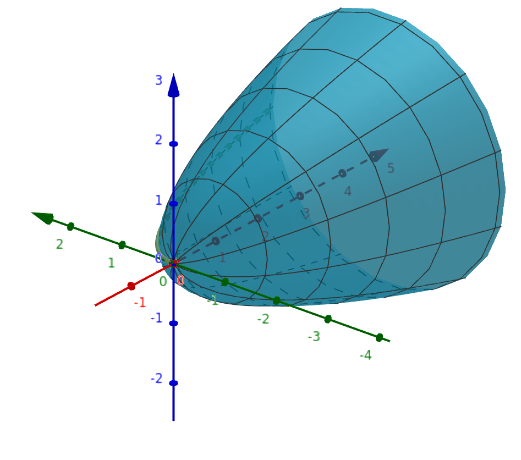
\includegraphics[width=7cm]{5L-1.3-could.be.mathijs.INF.png}
\end{figure}

$ = 2 \pi \bint_0^2 \sqrt{x + \dfrac{1}{4}} dx$\\

\textbf{Onbepaalde integraal:}\\

Neem $t = x + \dfrac{1}{4} \Rightarrow dt = dx$\\

$\bint_0^2 \sqrt{x + \dfrac{1}{4}} dx = \dfrac{2}{3}t\sqrt{t} + c = \dfrac{2}{3}\left(x + \dfrac{1}{4} \right) \sqrt{ x + \dfrac{1}{4} } + c$\\

$ = 2 \pi \left[\left(+\dfrac{1}{4}\right)\sqrt{x+\dfrac{1}{4}}\right]_0^2$\\

$ \dfrac{4\pi}{3}\left(\left(\dfrac{9}{4}\sqrt{\dfrac{9}{4}}\right) - \left(\dfrac{1}{4}\sqrt{\dfrac{1}{4}}\right)\right)$\\

$ = \dfrac{13 \pi}{3}$

\begin{thebibliography}{999}
\bibitem{} https://www.geogebra.org/m/r4gweqnt
\end{thebibliography}
\end{document} 
